\section{Verifying memory consumption} \label{sec:verification}
%Here we describe how to automatically check the annotations introduced in the previous section relying on \textsc{Code Contracts} verifier (\textsc{Clousot}). 
%
%Basically, we transform the annotated program into a functionally equivalent but instrumented in such way that the \textsc{Code Contracts} verifier is able to determine the correctness of the annotations.
To automatically check the annotations introduced in the previous section we transform the annotated program into a functionally equivalent program but instrumented into one using only \textsc{Code Contracts} annotations in such way  that a successful  verification of the transformed program implies the correctness of the original resource usage annotations.

\subsection{Introducing counters and ensure clauses}
%For verification purposes we will interpret the memory consumption annotations as ensures clauses. 
%The idea behind the counters and contracts instrumentation is to generate a set of counters (integer attributes in the method's class) that are incremented in the body of the method being instrumented and a transformation of the given memory contracts into \textsc{Code Contracts} native contracts so that the given assertions are expressed in function of the counters and can be verified by \textsc{Code Contracts}.
For every method \mono{m} featuring memory consumption we apply the following procedure:
let $T$ be the set of memory lifetime tags appearing in the contract (including one for temporary consumption) and $C$ the set of classes. For each tag $\mono{t} \in T$ and $\mono{C} \in C$ we introduce a counter \mono{C\_m\_t}   which tracks the number of objects  of type \mono{C}  from \mono{m}  that are associated with tag \mono{t}.
To keep the counters updated, for each  \mono{new C()} statement annotated with \mono{DestTmp} or \mono{DestRsd(t)}, we introduce a statement to increment  \mono{C\_m\_t}. 
Finally, the memory consumption annotations are transformed into corresponding ensure clauses stating that the associated counters are less than or equal to the specified bounds. 

Concretely:  \mono{Contract<C>.Rsd(t, e)} is transformed into \mono{Contract.Ensures(\mono{C\_m\_t} <= e)}. The same approach applies for  temporary consumption contracts.

%For each contract we will generate a counter, this counter will be incremented for each \textit{new} statement annotated with \mono{DestTmp} or \mono{DestRsd} where the destination of the object is the type of memory corresponding to the contract being instrumented. Then, the contract is transformed into a \mono{Contract.Ensures} annotation with an expression combining the counter and the integer expression given by the user.

% Lets see an example of this instrumentation. Given this simple method:
% 
% \vspace*{5pt}
% \begin{scriptsize}
% \begin{lstlisting}[caption=Example method not instrumented]
% public Person CreatePerson(string name)
% {
% 	Contract.Memory.Rsd<Person>(Contract.Memory.Return, 1);
% 	Contract.Memory.DestRsd(Contract.Memory.Return);
% 	return new Person(name);
% }
% \end{lstlisting}
% \end{scriptsize}
% \vspace*{5pt}
% 
% This is the same method instrumented:
% 
\begin{figure}[b]
%\vspace{1em}
 \begin{scriptsize}
 \begin{lstlisting}[numbers=none]
 public static int Person_CP_rsd_return;
 public Person CreatePerson(string name)  {
 	...
	Contract.Ensures(Person_rsd_return <= names.Count);
 	Person_CP_rsd_return = 0;
 	...		
	for (int i = 0; i < names.Count; i++)	{
		Person_CP_rsd_return++;
		Person p = new Person();
		Person_CP_rsd_return += Person_SI_this;
		p.SetInfo(names[i], address);
		...
 \end{lstlisting}
 \end{scriptsize}
 \vspace{-.5em}
\caption{Fragment of an instrumented version} \label{ex1-inst}
\end{figure}
% 
% With this instrumented code, the \textsc{Code Contracts} static verifier is going to try to verify the correctnes of the inserted contracts in line 5 and the result can be seen in the Visual Studio verification results along the \textsc{Code Contracts} results like Figure \ref{ex1} shows.

For the annotations \mono{AddTmp(d)} and \mono{AddRsd(d, s)} the instrumentation consists in adding to the respective local counters the value of the callee counter. 
%That way, \textsc{Code Contracts} will be able to determine the quantity of objects transferred from the callee using the instrumented contract the called method.

% Like we mentioned before, the \textit{temporal} memory of the called methods should be maximized and considered part of the required \textit{temporal} memory of the caller method for it to be safely executed. This is also done during the instrumentation phase using the method \mono{Math.Max} when adding to the counters, taking special care if it is done inside a loop.

The instrumentation is performed at the IL level and is never read or manipulated by developers.
Only for demonstration purposes, in Figure~\ref{ex1-inst} we show a fragment of the instrumented version of the  method presented in Figure~\ref{ex1}.

%For demonstration purposes, in Figure~\ref{ex1-inst} we show a fragment of the instrumented version of the  method presented in Figure~\ref{ex1}. Actually, the instrumentation is performed at the IL level and is never read or manipulated by developers.

\subsection{Verifying object lifetime annotations}
The instrumentation and verification process assume that object lifetime annotations \mono{DestTmp} and \mono{DestRsd} are correct. To ensure they actually are, we include a lifetime-annotations checker. 
Figure~\ref{ex2} shows an example where an escaping object is incorrectly declared as temporary. The squiggly highlights the position of that error.



To perform this verification we rely on a points-to and escape analysis capable of analyzing .NET programs~\cite{garber07iwaco}.  For every annotated method we run the analysis and build a points-to graph (PTG) which is basically an abstraction of the program heap visible from each method at the end of its  execution. To verify the correctness of \mono{DestTmp} annotation, we check whether the node in the PTG, representing objects created at that program point, is not reachable from the global scope, method parameters or the returned object.  For \mono{DestRsd} we check if the object escapes and it is reachable through the path expression associated with the tag (i.e.,  by using \mono{BindRsd}).
The correctness of the lifetime information associated to the annotations \mono{AddTmp} and \mono{AddRsd}, where the objects are transferred to the objects designated by the corresponding tags, is also verified in a similar fashion.

%Using an implementation of the algorithms defined in \cite{garber07iwaco} we do a points-to and escape analysis of the code and verify the correctness of the annotations \mono{DestTmp} and \mono{DestRsd}. 
\begin{figure}[tb]
% \fbox{
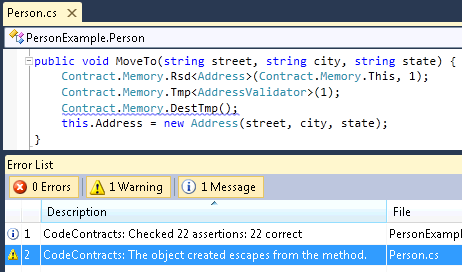
\includegraphics[width=1\linewidth, clip]{screen_verif_dest2.png}
%}
%\vspace*{-2em}
\vspace{-2em}
\caption{Lifetime annotations verification result}
\vspace*{-1em}
\label{ex2}
\end{figure}



\section{Verifying complex contracts} \label{sec:barvinok}
\textsc{Clousot} does a very good job in performing automatic verification of contracts, being able to check method featuring loops without demanding loop invariants. 
However, it has some limitations when dealing with the complex arithmetic required for a quantitative analysis. According to our experiments the current version of \textsc{Clousot} is restrained to contracts having linear integer expressions.
 %Another limitation found in the verification using \textsc{Clousot} is related to the usage of \mono{Math.Max}.} Just like with the contracts, the arithmetic module isn't able to handle non-linear expressions.

\textsc{Barvinok}~\cite{clauss2009symbolic} is a tool\footnote{\small Available at: \url{http://freshmeat.net/projects/barvinok}.} capable of manipulating parametric integer sets and relations.  It provides functionality to \emph{count} the number of elements of these sets and for performing \emph{maximization} and \emph{sum} on polynomials over these sets. 
Given a method featuring a loop (with possible several nested loops) including a \mono{new} statement  
and a predicate describing its iteration space (i.e. a linear restriction describing the relation between the loop inductive variables and parameters),  we can obtain a parametric upper-bound of the number of times the  \mono{new} statement is executed. This upper bound is obtained by counting the number of solutions of that iteration space~\cite{garber08ismm}. 
In a similar fashion, we can deal with polynomial temporary and residual consumptions by applying respectively a symbolic maximization and sum operations over the iteration space. 



For those methods whose consumption is beyond the capabilities of \textsc{Clousot} we can use this approach. The price to pay to obtain more precision is the need of a new annotation to specify iteration spaces inside loops: \mono{IterationSpace}. Although this increases the annotation burden,  the gain is considerable since it makes possible the verification (and inference) of polynomial consumption. 
Notice that iteration spaces are a set of linear constraints, amenable to  be checked with \textsc{Code Contracts} as well.
We think it will be possible to automatically generate these annotations leveraging  on \textsc{Clousot} abilities on inferring loop invariants.

\begin{figure}[hbt]
\begin{scriptsize}
\begin{lstlisting}
public List<Person> CreateBigFamily(int n) {
	Contract.Requires(n > 0);
	Contract.Memory.Rsd<Person>(Contract.Memory.Return,
															n*(n+1)/2);

	List<Person> family = new List<Person>(n*(n+1)/2);
	for (int i = 1; i <= n; i++) {
		Contract.Memory.IterationSpace(1 <= i && i <= n);
		for (int j = 1; j <= i; j++) {
			Contract.Memory.IterationSpace(1 <= j && j <= i);
			Contract.Memory.DestRsd(Contract.Memory.Return);
			Person p = new Person(); (*@ \label{ex3:new-2loop} @*)
			family.Add(p);
		}
	}
	return family;
}
\end{lstlisting}
\end{scriptsize}
\vspace{-.5em}
\caption{Using \mono{IterationSpace} to assist the prover}
\vspace{-1.5em}
\label{ex3}
\end{figure}

Figure \ref{ex3} shows a method with a loop and a nested loop inside it. In this case \textsc{Clousot} would not be able to verify the contract. 
However, using  \textsc{Barvinok} and the aid of  \mono{IterationSpace} annotations in the loops we can determine the exact number of times that the \mono{new} statement on line~\ref{ex3:new-2loop} is executed and instruct the engine with new knowledge.


%When methods get longer they tend to have several increments to the counters, and in that cases even if we always add to the counters pre-calculated expressions, the verifier isn't able to determine that the sum of all the expressions meets the contract. For these cases, we can also use \textsc{Barvinok} to help during the verification. We build an expression composed of all the expressions added to a counter and verify, using \textsc{Barvinok}, if this expression meets the given contract; if it does we give that information to the verifier introducing a \mono{Contract.Assume} statement, therefore adding this information to the verifier knowledge base and letting it verify the correctness of the contract.